%        File: enucatl.tex
%     Created: dom ago 23 10:00  2009 C
% Last Change: 
% mar ago 25 09:55:26 CEST 2009
%
\documentclass[italian,a4paper]{article}
\usepackage[text={6in,9in},centering]{geometry}
\usepackage[]{url}
\usepackage[footnotesize,bf]{caption}
\usepackage{graphicx,wrapfig}
\usepackage[utf8x]{inputenc}
\usepackage[T1]{fontenc}
\usepackage{babel,ae,aecompl}
\frenchspacing
\pagestyle{plain}

\begin{document}
\section*{Introduzione}
Questa storia nasce nei primi giorni del luglio 2007, come omaggio alle
produzioni del T9 di Nokia che, alla richiesta di scrivere ``il pendolo di
Foucault'' produsse ``il pendolo di Enucatl?''. L'innegabile suono
azteco del nome e l'atmosfera che si originava
dalla lettura del libro di Umberto Eco indusse a non tralasciare questo
segno divinatorio (si direbbe del nostro Abulafia) e a produrre queste tre
storie, che rimasero pubblicate su Wikipedia\footnote{Qui, la discussione
del bar di Wikipedia sul nostro lavoretto:  \\
http://it.wikipedia.org/wiki/Wikipedia:Bar/Discussioni/Possibile\_bufala\_in\_serie} per circa una settimana.
\begin{quote}
    Alcuni riferimenti bibliografici palesemente inventati mi rendono sicuro
    che si tratti di una burla anche se di ottima fattura. \\
    \begin{flushright}
    -- Cotton, ``patrollatore'' di Wikipedia
    \end{flushright}
\end{quote}
 

\section*{Enucatl}
\begin{wrapfigure}[19]{r}[0in]{.3\textwidth}
    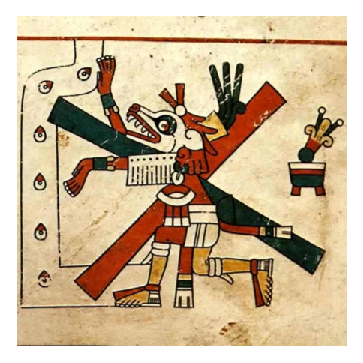
\includegraphics{enucatl.eps}
    \caption{Una raffigurazione di Enucatl (Codice \emph{Fejervary-Mayer}, XV
    secolo)}
\end{wrapfigure}
 Divinità facente parte della più antica mitologia azteca. \`E,
 nella tradizione riportata da numerose pergamene mesoamericane, il fratello
 di Quetzalcoatl, dal quale si distingue per la mancanza di piumaggio; è
 solitamente raffigurato nella forma di un serpente con ali di pipistrello,
 una tagliente coda biforcuta, una folta criniera sanguigna, un muso
 allungato di coccodrillo munito di micidiali zanne.

 Rientra nel gruppo della divinità ctònie, la sua qualifica principale è
 quella di Tauroboliaste e Psicopompo: suo compito precipuo, infatti, era quello di guidare
 le anime al Mictlàn, l'Oltretomba delle religioni precolombiane. Tuttavia,
 almeno stando alle leggende, non era raro che questa divinità, nota tra
 tutte le altre per la nobiltà d'animo, s'impietosisse delle anime che
 trasportava, consentendo ad esse di risorgere nei rispettivi corpi: simili
 eventi erano sovente accompagnati da mastodontiche scosse telluriche, e
 talvolta da possenti maremoti. Le ricerche dell'antropologo John C.
 Gnostolds (1898-1973), condotte nei pressi della Città Santa di Sobbabia,
 hanno portato alla luce numerose sepolture che non contenevano più
 cadaveri: una prova schiacciante (come ebbe modo di teorizzare nella sua
 opera maggiore, \emph{The ancient cult of Enucatl --- A scientific research on
 Mexican holy cities 1961-68}, edito nel 1970) della avvenuta resurrezione di
 massa.

 La cintura di templi che si dipana da Sobbabia fino a Tenochtitlan è
 riprova della devozione che il popolo azteco --- e, secondo alcuni artefatti
 rinvenuti nello Yucatan, anche maya --- nutriva nei confronti di questa
 divinità: si trattava di piramidi a gradoni smussati alte in media 45/60
 metri, in cima alle quali, per onorare il dio, venivano consumati sacrifici
 umani; con il declinare della potenza militare azteca, e il conseguente
 venir meno di schiavi, i templi della cintura delle Città Sacre furpono
 però abbandonati e andarono in rovina. Con essi sarebbe finito anche il
 culto del dio Enucatl (cfr. John C. Gnostolds, \emph{The ancient cult of Enucatl
 --- A scientific research on Mexican holy cities 1968-1973}, edito postumo
 nel 1980). Vi è da dire che Azazabe non fu l'ultimo Riverito Oratore della
 dinastia Mexica a celebrare solenni cerimonie nel complesso di Sobbabia;
 alla sua morte (1321) gli succedette il tiranno Mauro (1300-1322),
 condannato a una pressoché totale damnatio memoriae per la suprema
 efferatezza; pare che egli, riunito l'esercito e sconfitti in rapida
 successione i popoli confinanti, che avevano osato ribellarsi, abbia
 condotto almeno 10.000 prigionieri alla morte per onorare il dio Enucatl.
 
 I fedeli del dio-serpente resistettero, soprattutto nelle campagne, col
 nome di ajaxes; ma l'arrivo degli spagnoli, nel 1521, condusse alla
 distruzione della maggior parte dei documenti su Enucatl e alla definitiva
 cessazione del suo ricordo.
 Solo negli Anni Sessanta del Ventesimo Secolo le ricerche di John C.
 Gnostolds poterono restituire a questa antica divinità una parte della sua
 antica, e per sempre perduta, identità.
%
\section*{Tiranno Mauro}
 Riverito Oratore del popolo azteco (1300-1322), ebbe vita
 invero brevissima. A lungo condiserato poco meno di una figura
 leggendaria, ottenne la patente di storicità in seguito alle approfondite
 ricerche eseguite da John C. Gnostolds nella cintura dei templi, in
 Messico, e pubblicate nel suo libro \emph{Tyrant Maurus --- A history about
 Enucatl's legacy XIV Century to XX}.
 \subsection*{L'infanzia e il culto di Enucatl}
 Nato da Nahuatl, comandante dell'esercito di Tenochtitlan, e dalla
 principessa Hemutillin, cugina dell'allora re Azazale, per la lontananza di
 parentela dal sovrano, sembrò fin da subito escluso dalla successione al
 trono.

 L'incontro con il culto del sanguinario dio Enucatl, già a nove anni,
 cambiò radicalmente la sua vita: avvenuti al termine di una travagliata
 crisi mistica, nel corso della quale Mauro si sarebbe inflitto pesanti
 automutilazioni e avrebbe avuto visioni dell'aldilà, l'adesione alla setta
 che onorava questa divinità e l'ingresso nei Santi Misteri plasmarono il
 suo carattere ancora giovanissimo. In breve, sorretto in ogni sua azione
 dalla cieca fede in Enucatl, divenne audace, spregiudicato, protervo; a
 dodici anni convinse suo zio Azazale ad inviarlo nella Città Santa di
 Sobbabia per un tirocinio sacerdotale, vincendo l'opposizione di sua madre
 (suo padre, nel frattempo, era caduto in battaglia contro i vicino
 Tlaxcaltechi): preso sotto l'ala protettrice di un Sommo Sacerdote noto
 solo come Fiore Ascetico, crebbe nel più acceso e settario fanatismo
 religioso, giungendo a convincersi della possibilità di unificare tutto il
 popolo azteco e le popolazioni confinanti sotto un unico dio, che, se del
 caso, doveva essere imposto an che con la violenza.
 \subsection*{La carriera militare e l'ascesa al potere}
\begin{wrapfigure}[18]{r}[0in]{.3\textwidth}
    
\includegraphics[width=.4\textwidth]{tirannomauro.eps}
    \caption{Una delle poche statue del tiranno scampate alla furia
    iconoclasta che segu\`i alla fine del suo regno.}
\end{wrapfigure}
 A quindici anni, Mauro ottenne l'esenzione dalla frequenza scolastica e
 l'ingresso nell'esercito: si addestrò febbrilmente per due anni e, come
 tributo per il grande coraggio e la cieca abnegazione, gli fu assegnato il
 comando di una numerosa guarnigione di frontiera, collocata al limitare del
 territorio tlaxcalteco. Approfittando della sua condizione di ``quasi re''
 nella guarnigione, indusse i suoi uomini ad abiurare la Fede Tradizionale,
 riconoscendo come unico dio Enucatl; i pochi che, di fronte al suo zelo
 fanatico, ebbero la forza di opporsi, vennero sottoposti a una tortura
 divenuta poi famosa come ``tortura del Tiranno'': crocifissi a testa in giù,
 dopo che era stata loro strappata la lingua, venivano affogati a più
 riprese in tinozze d'acqua bollente. Una simile politica di conversioni
 forzate fu seguita anche per i vicini villaggi tlaxcaltechi, molti dei
 quali vennero completamente rasi al suolo per aver rifiutato il nuovo dio;
 ormai i guerrieri della guarnigione al comando di Mauro agivano solo su suo
 ordine, trascurando i dispacci che provenivano dalla capitale, massacrando
 le popolazioni inermi e convertendo in massa i sopravvissuti. Quel ch'è
 più, molti guerrieri, provenienti da guarnigioni diverse o da molto tempo
 lontani dal campo di battaglia, si convertirono spontaneamente ed entrarono
 al servizio di Mauro, che ormai poteva contare su oltre 3.000 uomini.
 Alla morte di Azazale, nel giugno 1319, seguirono sei mesi di anarchia: la
 mancata associazione al trono di un qualsiasi erede e il ritardo del
 collegio sacerdotale nello sceglierne uno, com'era sua competenza, indusse
 diversi generali, tra cui anche il buon Satrapàme, ad autoproclamarsi re,
 contando sul sostegno dei propri soldati. La notte del 31 dicembre 1320
 (detta anche Notte delle Canne), Mauro marciò sulla capitale Tecnochtitlan,
 sostenuto da una folla osannante, sconfisse due dei generali che,
 coalizzatisi, gli sbarravano la strada ed entrò in Tenochtitlan, dove
 ordinò l'abbattimento delle statue dei ``falsi idoli'', e decise di
 sacrificare chi, tra i prigionieri di quella notte, non si fosse sottomesso
 e convertito. Morirono a migliaia.
 \subsection*{Il regno del Tiranno Mauro}
 Nel marzo 1320 Mauro fu costretto, per un'epidemia che aveva colpito
 Tenochtitlan, a raggiungere un compromesso con l'ultimo usurpatore rimasto,
 il buon Satrapàme: in cambio del riconoscimento della regalità di Mauro,
 quello avrebbe ottenuto la mano di sua sorella Tzitziplin, appena
 dodicenne, e sarebbe stato associato al trono. Dopo nove mesi, l'anarchia
 militare aveva fine.

 Iniziò, però, una nuova stagione di violenze: la furia iconoclasta di Mauro
 si abbatté su monumenti, templi e recinti sacri degli altri dèi; la
 ``tortura del Tiranno'' venne inflitta spietatamente e reiteratamente a
 nemici e sudditi; i regni tlaxcaltechi furono sottomessi e i 10.000 loro
 prigionieri, fedeli alle antiche tradizioni, vennero immolati sulla
 piramide di Enucatl, nella Città Santa di Sobbabia --- secondo le cronache,
 furono necessari sette giorni di massacro ininterrotto. La pressione fiscale,
 inoltre, levitava per la necessità di sostentare un esercito sembre più
 agguerito e sempre più feroce.

 Nelle campagne, il culto si radicava profondamente: i fedeli del
 dio-serpente, detti ajaxes, non di rado assaltavano le città sguarnite di
 fortificazioni imponendo la conversione alle borghesie mercantili e
 artigiane di città. Infine, l'epidemia che aveva colpito Tenochtitlan non
 era ancora stata debellata, e i canali della città erano ingombri di
 cadaveri in decomposizione.

 La situazione, nei due anni in cui regnò il tiranno Mauro, si fece
 insostenibile: l'intolleranza religiosa, le conversioni forzate, le
 torture, i massacri nelle campagne e nelle città, la pressione fiscale
 esagerata, le continue guerre con Chichimechi e Tlaxcaltechi indussero il
 buon Satrapàme, cognato di Mauro, a rovesciarlo, il 14 luglio 1322; quel
 giorno fu noto come Giorno della Gloria. L'evangelizzatore violento del
 culto di Enucatl, incatenato e sconfitto, abbandonato da tutti, fu l'ultima
 vittima offerta al dio-serpente; questa religione, intollerante e violenta,
 fu dunque messa al bando per sempre --- anche se, come affermano documenti
 spagnoli del XVI secolo, persistette lungamente nelle campagne, perpetuato
 dagli ajaxes.
 \subsection*{Definitivo declino e \emph{damnatio memoriae}}
 I monumenti che il tiranno Mauro aveva fatto erigere, le sculture che lo
 ritraevano, i dipinti che celebravano le sue vittorie furono immediatamente
 distrutti; il suo nome, cancellato da ogni registro del Paese, fu
 dimenticato: la condanna per i suoi efferati atti fu così la perenne
 \emph{damnatio memoriae}. Talché il suo nome, Mauro, non è azteco: furono gli
 spagnoli a tradurre così, fraintendendo, l'aggettivo \emph{mah-urr} (nero
 d'animo) con cui egli veniva descritto da una popolazione, a distanza di due
 secoli, ancora terrorizzata.
 %
 \section*{Satrapame (conosciuto come il Buono)}
 Riverito Oratore azteco dal 1322
 al 1351, noto, tra i numerosi sovrani aztechi, per aver posto fine al
 Sacri Misteri regolarmente celebrati in onore del dio Enucatl e alla
 furia inconoclasta che il suo predecessore, il tiranno Mauro, aveva
 scatenato nei confronti delle altre divinità.
 \subsection*{La guerra civile}
 Alla morte di Azazale, nel 1319, il buon Satrapàme aveva appena
 quarantacinque anni, ma già da dieci comandava 5.000 guerrieri induriti
 dalle battaglie, rigidamente disciplinati e fedeli al loro comandante, che
 si atteggiava a signorotto feudale di un'inospitale zona del deserto di
 Bradorose, al confine più settentrionale dell'Impero Azteco.
 La notizia della fine del monarca giunse provvidenziale: c'è chi sostiene
 (in particolare Edward J. Gnostolds, figlio del più celebre antropologo
 John C. e prosecutore delle sue ricerche, in \emph{Tyrant Maurus and the Good
 Satrapames --- Anarchy and civil war in the Ancient Mexico}) che il sovrano
 improvvisamente deceduto fosse al corrente dei traffici che il buon
 Satrapàme intratteneva con le popolazioni autoctone oltre il confine
 dell'Impero --- semi di cacao, pietre preziose, armi, piante allucinogene --- e
 che si preparasse a guidare un esercito contro il suo vassallo infedele.
 Appena informato della vacanza del trono, il suo esercito personale lo
 acclamò imperatore (4 luglio 1319): documenti dell'epoca attestano una sua
 esitazione di fronte alla corona che gli veniva offerta, risolta
 positivamente in seguito alla scoperta della ribellione del futuro tiranno
 Mauro.
  
 Seguirono sei mesi di guerra civile, un periodo di anarchia militare nel
 quale cinque autoproclamatisi imperatori si affrontarono in sanguinose
 battaglie delle quali non ci sono giunte notizie dettagliate; è un fatto
 che nella Notte delle Canne (31 dicembre 1319) il tiranno Mauro riuscì a
 impadronirsi con un abile colpo di mano della capitale Tenochtitlàn, e che
 solo per un'epidemia, che aveva messo in ginocchio la città, lo scontro fra
 le truppe di Mauro e Satrapàme fu evitato. L'accordo, stilato tra i due
 usurpatori, prevedeva che Satrapàme riconoscesse la regalità del rivale; in
 cambio avrebbe sposato sua sorella Tzitziplin, di appena dodici anni, e
 sarebbe stato nominato erede al trono.
 Satrapàme accettò di buon grado.
 \subsection*{Il regno del buon Satrapame}
\begin{wrapfigure}[22]{l}[0in]{.3\textwidth}
    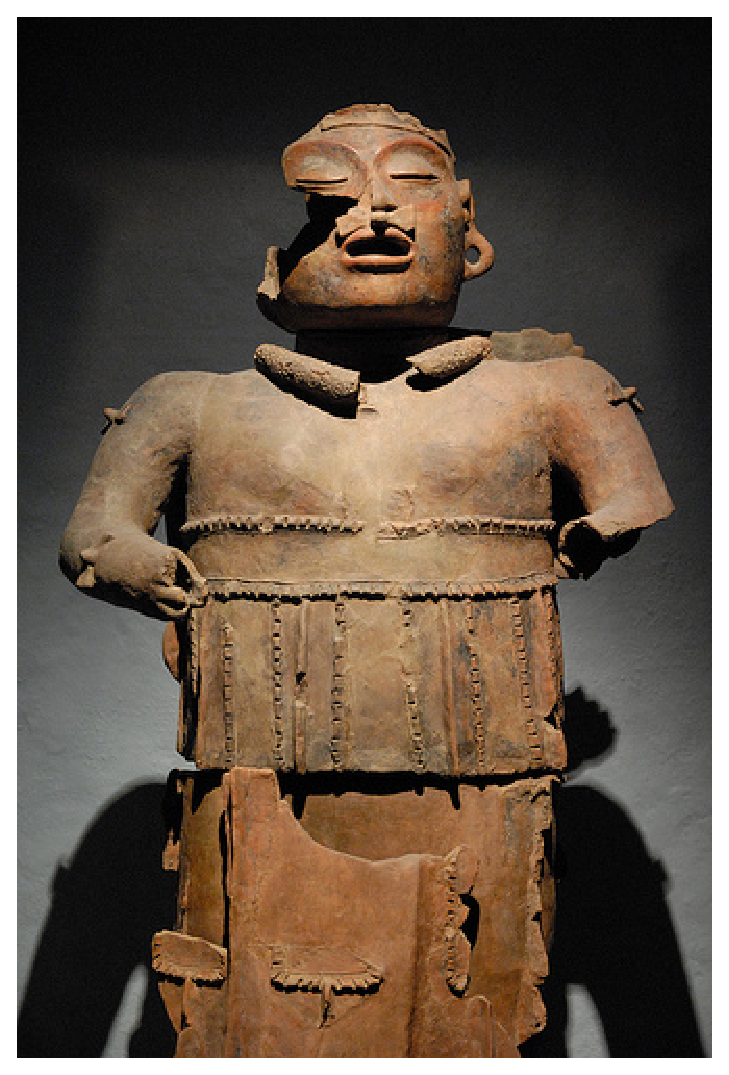
\includegraphics[height=.3\textheight]{satrapame.eps}
    \caption{Una statua del buon Satrapame,
    conservata nel museo del Templo Mayor, a Città del Messico.}
\end{wrapfigure}
 Nei mesi seguenti, però, il crescente odio
 delle masse popolari contro le politiche d'intolleranza religiosa del
 tiranno Mauro lo indusse a rovesciarlo il 14 luglio 1322 (Giorno della
 Gloria); il desposta deposto fu sacrificato sull'altare di Enucatl e il
 culto bandito per sempre.
 Avevano così inizio ventinove anni di governo illuminato: il buon Satrapàme
 ampliò le fortificazioni già appartenutegli, sul confine settentrionale,
 per difendere l'Impero dalle orde di selvaggi che premevano con insistenza
 alle frontiere; un loro tentativo velleitario di forzare queste difese
 indusse il generale Cuahumatl, comandante dell'élite guerriera dei
 Cuahchiqueh e amico intimo del buon Satrapàme, ad attaccare il nemico. Uno
 scontro di proporzioni epiche vide opporsi 1.000 guerrieri aztechi a oltre
 ventimila stranieri, e riportare su questi ultimi una vittoria
 schiacciante. I prigionieri --- pochi, a dir la verità --- vennero immolati
 sulle fortificazioni il giorno della loro inaugurazione.

 Satrapàme premiò Cuahumatl associandolo al trono; voci insistenti, raccolte
 dall'archeologo Jean-Pierre Donatien (\emph{Homosexualité et amour chez les
 Azthèques}), parlano di una realazione omosessuale tra i due. Tzitziplin, la
 moglie del Riverito Oratore, si era intanto rivelata sterile: fu uccisa in
 gran segreto, il suo corpo gettato nei canali di Tenochtitlàn.
 Ma l'opera del sovrano illuminato non si arrestò qui: egli ordinò
 l'ampliamento e la difesa delle vie di comunicazione con lo Yucatan, e
 inviò diverse missioni esplorative fino alla costa dell'Oceano Pacifico.
 Fece erigere numerosi templi al dio Quetzalcoatl, invocandone il suo
 ritorno dal Mare Occidentale; stabilì un'alleanza, destinata a durare solo
 un ventennio, con i vicino Tlaxcaltechi, grazie alla quale poté condurre
 guerre di conquista nel meridione del Paese.
 Rinnovò il calendario, stabilendo che cinque giorni venissero aggiunti ogni
 vent'anni per evitare un'eccessiva discrepanza tra le previsione matematica
 e lo scorrere delle stagioni. Emanò diversi editti, volti a contenere la
 pratica del duello, molto diffusa --- anche se, pare, non ebbe molto
 successo; sempre sul piano legislativo, raccolse in un unico corpo,
 suddiviso in dieci libri, antiche tradizioni religiose e giuridiche del
 proprio popolo.
 \subsection*{Follia e morte in disgrazia}
 Negli ultimi anni della sua vita, la follia lo assalì; mise a morte la sua
 nuova moglie, Hematlel, che lo aveva accusato pubblicamente di impotenza
 (1347); fece fustigare tutti i servi della casa reale perché non erano
 stati in grado di recuperare un bracciale che aveva perduto; fece mettere a
 ferro e a fuoco le case degli oppositori politici, che con la sua pazzia si
 facevano sempre più audaci e lanciavano in pubblico i loro anatemi; iniziò
 a sospettare persino dell'ostilità del generale Cuahumatl, il quale,
 temendo di soccombere, mobilitò i suoi guerrieri per attaccare il palazzo
 reale. Nel 1351 il buon Satrapàme fu deposto e incarcerato; Cuahumatl non
 si proclamò re, ma impose sul trono il giovane e manovrabile Cajalcoyotl,
 di cui avrebbe continuato a essere l'eminenza grigia per i successivi
 dodici anni. Satrapàme, cieco e folle, morì dopo quattordici giorni di
 prigionia.
\end{document}
